\section{Coster}
\label{subs:coster}

%\begin{figure}[h]
%\centering
%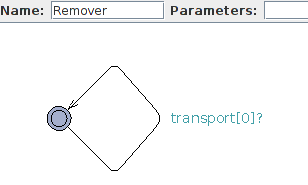
\includegraphics[width=0.6\textwidth]{firstremover.png}
%\caption{The model of the remover template}
%\label{fig:firstremover}
%\end{figure}

%The \emph{coster template} ensures that parallel processing of recipes is prefered, during a best-first Search. It can be seen in \cref{fig:firstcoster} The \emph{coster template} is initialised with a rate \emph{c}, which increases the \emph{cost} variable as a function of the global time passed. Without this, the search would not have any reason to run several modules at the same time as the final \emph{cost} would not change. By having a constant \emph{cost} on the factory’s operating time, we make the prospect of parallel processing a prefered option.
